\documentclass[a4paper,12pt]{article}
\usepackage{fancyhdr}
\usepackage{geometry}
\usepackage{setspace}
\usepackage{graphicx}
\usepackage{amsmath}
\usepackage{amsfonts}
\usepackage{algorithm}
\usepackage{algorithmicx}
\usepackage{wrapfig}
\usepackage{indentfirst}

%To Do: 
%	[X] Spruce up Abstract, Spruce up background (what mri is, relaxation times, maybe include graphs of exponentially dependent functions) 
%	[?] Reword some of Canny Edge Detection section (use source Ed sent me), maybe include visuals of binning, gradient directions, and such
%	[?] Add to design of system (mention synced folders briefly, and directory formats), and concentration
%	[3] Add to Synthesis of MnCl
%	[3] Sprinkle some citations in the Results
%	[3] Spruce Up Results for Sample Goodness w/ Edge Detection
%	[]		Issues: Noise and Such, Confidence about Sample's goodness
%	[3] Write about Results with most optimal conc
%	[] 		Include a sample of pure agar? See what happens!
%	[1] Conclusion: Results Discussion, Future Applications

\setlength\parindent{24pt}

\doublespacing

\begin{document}
	\begin{center}
	\vspace{0.5cm}
	\huge{Applications of Image-Analysis \& Canny Edge Detection in Manganese-Enhanced Magnetic Resonance Imaging}\\
	\vspace{0.5cm}

	\singlespacing
	\small{Patrick C. Stocklin}\\

	\small{Advisor: Edward Van Keuren}

	\small{Georgetown University}\\

	\small{4/24/16}\\
	\end{center}

\begin{section}{Abstract}
\singlespacing

Magnetic Resonance Imaging is an imaging technique used to render images from differing magnetization-vector relaxation times of hydrogen proton's found in organic tissue. By applying a constant magnetic field, the protons' magnetization moments are excited and precess about the field's axes. When hit by a radio frequency pulse, they are excited into a high energy state, then return to their lower energy states and emit electromagnetic energy. MRI contrast agents alter the differences in these relaxation times by introducing miniscule magnetic fields surrounding the hydrogen-proton. This paper discusses the applications of digital image-analysis techniques, like Canny edge detection, towards computing the effectiveness of manganese-based contrast agents in MRI. The fall semester was spent investigating feature-extraction techniques in image-analysis. Professor Van Keuren and I both turned our attention towards Canny edge detection, in hopes that it would yield promising applications and precious information related to our research. The spring semester was more focused on the results and applications of image-analysis on manganese chloride contrast agents. Many samples of manganese chloride, each with varying concentration levels, were made and imaged to discover more about these promising $T_1$ and $T_2$ contrast agents. The spring semester was spent constructing an open-source Linux-based environment to analyze MRI images and create algorithms which determine the most effective concentration level for a manganese-based contrast agent.

%Add about what was found

\end{section}

\newpage
\doublespacing
%%%Things to Add for Sources:
%%%Pictures of Different Thresholds
%%%1D case for gradients.http://suraj.lums.edu.pk/~cs436a02/CannyImplementation.htm
%%%Modeling Intensity Changes (step edge, sharp edge, roof edge, ridge edge)
%%%Roberts, Prewitt, Sobel


\begin{section}{Background Information}

%MRI INFO FROM BRADY/OXFORD SLIDES
%T1-weighted image TR=14ms, TE = 50ms,
%T2-weighted image TR=4000ms, TE = 100ms
%H protons with two spin states are either precessing along or against the external magnetic field
%Bombarded with RF energy, at certain resonant (larmor) freqs the proton flips to high energy states
%Applying pulse at 90 degrees to the B field

%Relaxation T1
%For nuc to return to low energy states the spin system must be exposed to an EM field oscillating with a freq at or close to Larmor freq
%This can occur by the nuc being stimulated by surrounding nuc, occurs in exponential manner
%corresponds to the time req for the system to return to 63 percent of eq when exposed to 90 deg

%Saturation Recovery of Mz back to Mo

%Contribution of all spins is tipped into x,y plane, dephases in the x,y plane

%Relaxation T2, 
%immediately after pulse is applied, spins dephase and signal decreases
%Approximately 10x smaller than T1

%Maybe mention K space and FFT


\subsection{Magnetic Resonance Imaging}
Magnetic Resonance Imaging (MRI) is an imaging techinique used to visualize the anatomy and physiological topology of living organisms. By using powerful externally-applied magnetic fields, scientists and physicians are able to render detailed images of the human body without exposing the patient to potentially lethal forms of radiation. It is this exact reason why magnetic resonance imaging is the predominantly-favored investigative tool for detecting cancerous cancer cells. MRI is generally agreed upon to be superior to Computed Tomography (CT) scans for neurobiological visualization because it avoids any harmful exposure to radiation and offers a more detailed image of the grey and white matter in the central nervous system$\cite{1}$.
MRIs also allow for a multitude of images to be taken over a short span of time and may be used to monitor neural or vascular activity as the subject is placed under time-varying conditions or stimulation$\cite{1}\cite{2}$.
Thus it is said to be the leading imaging technique for neuroimaging. \\

\subsubsection{MRI Procedure}
Because the human body is mostly comprised of water molecules containing single protons in the nuclei of the Hydrogen atoms, MRI has proven to be an effective means of rendering anatomical images. The hydrogen protons within the area of interest are placed under with a strong, constant magnetic field.
Most clinical MRI machines typically operate between 0.7 - 2.0 Teslas$\cite{3}$. 
The protons' magnetic moment is temporarly altered, precessing about the direction of the applied magnetic-field $\cite{2}$. 
A radio frequency pulse is then simultaneously applied to the patient, exciting the protons into a high energy state. After a short interval of time, the protons return to their lower energy state and release electromagnetic energy.
This precession then yields a momentary change in the magnetic flux through the hydrogen atom, which creates a signal that the MRI scanner interprets. The collection of signals are then processed according to their respective frequencies emitted and the final produced image is obtained by applying a 2-D Fourier transformation across the spatial-frequency domain (k-space). 
The signal frequency is directly proportional to the period of time it takes for the protons to return to their low-energy equiilibrium state. This is known as the relaxation period $\cite{3}$. 
More specifically, the recovery of the longitudinal component of the proton's magnetization is classified as $T_1$ relaxation. This is essentially associated with the number of Hydrogen nuclei with parallel spin versus the number of nuclei with anti-parallel spin $\cite{3}$. 
The loss of phase coherence in the proton's transversal plane is responsible for the transversal relaxation, known as $T_2$ relaxation. This relaxation time is associated with the number of hydrogen nuclei in phase with each other $\cite{3}$. 
Both $T_1$ and $T_2$ relaxation rates govern the time it takes for the protons to fully return to equilibrium.


\newpage
\subsubsection{$T_1$ Relaxation}
$T_1$, or {\em Spin-Lattice Relaxation Time}, is the time required for the magnetization vector to recover 63 percent ($[1-(\frac{1}{e})]$) of its initial longitudinal magnetization after being struck with a radio-frequency pulse. It characterizes the exponential rate at which the longitudinal component of magnetization reaches equilibrium $\cite{3}$. This value is dependent on the hydrogen proton's environment and can be altered by the presence of ferromagnetic or paramagnetic particles $\cite{3}$. The longitudinal component of magnetization may be defined by the following time-dependent equation:

\begin{center}
$M_Z(t) = M_{Z,Eq}(1 - e^{-\frac{t}{T_1}})$ 
\end{center}

%Ed says I may have to include more information for this section
An MRI image may be $T_1$-weighted by adjusting the {\em Echo Time}, $T_E$, and {\em Repitition Time}, $T_R$, such that the values obey a conventional spin-echo sequence $\cite{4}$. The {\em Echo Time} may be thought of as the time period following excitation which the proton's signal is read $\cite{4}$. The {\em Repitition Time} may be described as the amount of time that exists between successive pulses of signal. The two times may be adjusted to heavily favor a $T_1$ signal and reduce the amount of contribution by the $T_2$ signal $\cite{4}$. By setting these short $T_R$ and $T_E$ times (typically on the order of $< 750$ ms and $< 40$ ms, respectively), the image will heavily favor image contrast caused by the longitudinal component of magnetization $\cite{4}$.

\subsubsection{$T_2$ Relaxation}
$T_2$, or {\em Spin-Spin Relaxation Time}, is the time required for the transverse component of magnetization to return 37 percent ($\frac{1}{e}$) of its initial magnetization. $T_2$ relaxation typically occurs more quickly than that of Spin-Lattice Relaxation Times $\cite{4}$. Like $T_1$, $T_2$ is dependent on the hydrogen-proton's environment. The transverse component of magnetization may be defined by the following equation:

\begin{center}
$M_{XY}(t) = M_{XY}(0)e^{-\frac{t}{T_2}}$ 
\end{center}

%Ed says "Also Point Out that T1 and T2 are characterized by measuring different magnetization directions (not just changing echo times)"

$T_2$-weighted images may be derived by selecting a $T_E$ that is on the order of the contrast agents {\em Spin-Spin Relaxation Time}. This reduces the information gained by $T_1$ because the excited protons' spins are now allowed to return to equilibrium before excitation $\cite{4}$.

\subsubsection{Contrast Agents}

The varying brightness contrast in the produced images is caused by the difference in the strength of the nuclear magnetic resonance signals recovered from the detectors. 
%Different types of tissues -> different T1 T2 naturally occuring contrast
This is dependent on the difference between the two relaxation times of the nuclei within the sample. Because of the difference between the longitudinal and transverse relaxation times, doctors observe an enhanced or decreased brightness of the sample due to the proton's local environment. In MRI scans, $T_1$ relaxation weighting will characteristically render white matter as white pixels$\cite{3}$. Gray matter within the examined region will appear gray$\cite{3}$. All cerebrospinal fluid, the clear colorless fluid that protects the brain matter, will appear black$\cite{3}$. However, sometimes the contrasting brightness between the types of brain matter will not be as profound or apparent. Therefore, scientists will typically employ the use of a contrast agent to induce a much brighter or darker signal. Because the process from which the MRI images are produce largely depends on the magnetic properties of the environment surrounding the water molecules, contrast agents are usually chosen for their magnetic properties$\cite{4}$. 

For the majority of this paper, we will be concerning ourselves with manganese chloride as our contrast agent of interest. Despite being in its infancy as an effective contrast agent, manganese-based paramagnetic particles have been proven to enchance the $T_1$ signal of MRI scans $\cite{5}$. Manganese ions ($Mn^{2+}$) are popular contrast agents in the use of MEMRI (Manganese-Enhanced Magnetic Resonance Imaging) $\cite{5}$. It had even been discovered that natural products with a high concentration of manganese can be used for increasing $T_1$ signal $\cite{6}$.

\subsection{Previous Work Done}
Previous work done by Professor Edward Van Keuren in collaboration with the Georgetown University chemistry and physics departments, and the Georgetown Lombardi Comprehensive Cancer Center has made great progress in the exploration for biocompatible nanomaterials as useful contrast agents for MRI. Professor Van Keuren's research team has explored the synthesis of copolymers based on the metal-oxo cluster $Mn_8 Fe_8 O_{12}(L)_{16}-(H_2 O)_4$, where L is an acetate or vinyl benzoic acid, coupled with styrene\cite[p.~9040]{7}. The cluster's relaxivity was examined using NMR and confirmed $Mn_8 Fe_8 O_{12}(L)_{16}-(H_2 O)_4$ to be a promising $T_2$ contrast agent. The cluster was also determined to have low cytotoxicity when studied on human prostate cancer cells, potentially allowing it to be used {\em in vivo} for MRI scans\cite[p.~9040]{7}. Testing had also been done on the paramagnetic nanobeads produced by the metal-oxo cluster $Mn_8 Fe_4 - (VBA)_{16}$ copolymerized with styrene. The nanobeads had been confirmed as a potentially useful $T_1$ contrast agent, as their effect on the relaxivity within a polymer matrix only altered the transverse relaxation time ($T_2$) and hardly affected the longitudinal relaxation time ($T_2$)\cite{7}.

More recently, there has been on-going research between the Lombardi Comprehensive Cancer Center and Georgetown University to determine the effect of particle shape and size on $T_2$ relaxation in contrast agents. Iron oxide nanoparticles had been discovered as promising $T_2$ contrast agents due to the inhomogeneous magnetic fields they produce $\cite{8}$. Previous research had proven that up to a critical point, the particle size directly alters the $T_2$ of ferromagnetic particles $\cite{8}$. This specific research explored three different particle contrast agents: 1) spherical magnetite ($Fe_3 O_3)$, 2) prolate magnetite, and 3) oblate barium ferrite ($BaFe_{12}O_{19}$). All particles were modeled as spheroidal, and samples consisted of varying concentration levels of contrast agents suspended in layers of 3 percent agar. It was confirmed that the size of the contrast agent did influence the relaxation time up to a point, but it was observed that the oblate-shaped barium ferrite agent had possessed a relaxivity that surpassed the theoretical limit plotted against surface area per volume $\cite{8}$. Thus the oblate $BaFe_{12}O_{19}$ could prove useful as an effective $T_2$ contrast agent $\cite{8}$.

%\begin{wrapfigure}{R}{0.3\textwidth}
%\begin{center}
%\centering
%\includegraphics[width=0.425\textwidth]{imageregistration.png}
%\caption{registering an image}
%\end{center}
%\end{wrapfigure}

\subsection{Canny Edge Detection}

In order to highlight the regions of an MRI image where a contrast agent may brighten or darken the signal, we tailored the process of Canny edge detection to MRI. Discovered by Australian computer scientist John F. Canny in 1986, Canny edge detection is a multi-stage algorithm used to detect a wide range of object-edges in any given image$\cite{9}$.
This particular edge-detection approach attempts to both minimize the low error rate at which it finds edges (find as many as possible) and suppress as much background noise as possible, so as to not produce spurious edges. Canny edge detection is used in many domains of image-analysis, as it allows for massive amounts of data reduction by extracting only the useful and interesting bits of information. Among all edge detection methods, Canny's implementation is by far the most popular and reliable algorithm to date because it satisfies the three criteria for edge detection by means of calculus of variations$\cite{10}$:\\

\singlespacing
\begin{enumerate}
\item Low error rate for detection edges, the algorithm should detect as many edges as possible  $\cite{11}$.
\item The edge points extracted from the algorithm must be localized to the center of the edge  $\cite{11}$.
\item Any given edge must only be marked once and image noise must not create spurious false images  $\cite{11}$.
\end{enumerate}
\doublespacing

To achieve this, Canny edge detection requires several steps: 1) smooth the image in order to reduce noise by applying an arbitrarily sized Gaussian filter across the intensity pixels, 2) calculate the gradient of the intensity pixels, 3) reduce the possibility of creating false edges by applying a non-maximum suppression to the image, 4) determine the potential edges by applying a "double threshold", and remove all other weak edges that are not connected to strong ones (Hysteresis). The required steps will now be elaborated upon in greater detail $\cite{12}$.

\subsubsection{Applying the Gaussian filter}

Due to the inherently chaotic and erratic nature of the process of MRI scans, naive edge-detection would be susceptible to false positives (detecting unnecessary or weak edges due to unsuppressed image noise). Therefore it is essential to minimize the potential for this accidental detection by smoothing the intensity matrix of our image by masking each pixel with a Gaussian filter$\cite{13}$.%%%%%%%%%
By masking each pixel of our image's intensity matrix, we effectively smooth the image matrix and reduce the amount of noise that may poorly influence our edge detection's results. For a Gaussian filter with kernel size $(2k+1)\times(2k+1)$: our convolution mask may be defined as$\cite{13}$:\\%%%%%%%%%%%%%
\begin{center}
$H_{ij} = \frac{1}{2\pi\sigma^{2}}^{-\frac{(i-k-1)^2+(j-k-1)^2}{2\sigma^2}}$
\end{center}

It is left to the researcher to determine the size of the Gaussian mask.
However it is important to note that as the size of the Gaussian filter increases, the detector's sensitivity to background noise falls off.
For the sake of a visual example, below is included a Gaussian filter for $\sigma = 1.4$ and of size $5\times5$:\\

\singlespacing
\begin{center}
$A_{GF} = \frac{1}{159}\begin{bmatrix}
	2	&	4	&	5	&	4	&	2\\
	4	&	9	&	{12}	&	9	&	4\\
	5	&	{12}	&	{15}	&	{12}	&	5\\
	4       &       9       &       {12}    &       9       &       4\\
	2       &       4       &       5       &       4       &       2
\end{bmatrix}$
\end{center}
\doublespacing

\subsubsection{Calculating the Intensity Gradients}

After smoothing our image to reduce background noise, the next step of Canny edge detection is to calculate the intensity gradients of all image pixels. Given an image matrix of intensity pixels, edges within the image are most likely to be found when there is a strong, well-defined gradient along a uniform direction. This distinguishes what a real-world edge is digitally. In order to achieve this, a 2-D gradient operator is selected to determine the intensity gradient of each pixel. There are several operators available to calculate the gradients, but the most popular is the $Sobel$ $operator$$\cite{14}$.%%%%%%%%%%%%%%
The 2-Dimensional Sobel operator $|G|$ is a pair of $n\times n$ convolution masks which estimate the gradient in the x and y directions. The Sobel operator allows us to find the edge strength (gradient) according to $|G|$ = $|G_x|$ + $|G_y|$, where $G_x$ and $G_y$ for mask size 3 are shown below:

\singlespacing
\begin{center}
\[G_x = 
\begin{bmatrix}
-1 & 0 & 1\\
-2 & 0 & 2\\
-1 & 0 & 1\\
\end{bmatrix}
, G_y =
\begin{bmatrix}
-1 & -2 & -1\\
0 & 0 & 0\\
1 & 2 & 1\\
\end{bmatrix}
\]
\end{center}
\doublespacing

Now that the horizontal and vertical gradients of our intensity pixels have been determined, calculating the edge gradient is fairly simple.
The edge gradient may trivially be calculated as $\textbf{G} = \sqrt{(G_x)^2 + (G_y)^2}$. 
The direction of the image gradient may be calculated using $atan2$, a trigonometric arctan function which takes in two function parameters and returns an angle from $(-\pi,\pi]$.
However, $atan2$ can be mapped to a range of $[0,2\pi)$ by adding a factor of $2\pi$ to all negative results.
In terms of the typical arctan function, $atan2(y,x)$, for $G_y$ and $G_x$ may be defined as below:

\singlespacing
\begin{center}
\[
atan2(G_y, G_x) = \left\{\def\arraystretch{1.2}%
  \begin{array}{@{}c@{\quad}l@{}}
	arctan(\frac{G_y}{G_x}) & \text{if $G_x$ $>$ 0,}\\
	arctan(\frac{G_y}{G_x}) + \pi & \text{if $G_x$ $<$ 0 and $G_y$ $\geq$ 0,}\\  
	arctan(\frac{G_y}{G_x}) - \pi & \text{if $G_x$ $<$ 0 and $G_y$ $<$ 0,}\\
	+\frac{\pi}{2} & \text{if $G_x$ = 0 and $G_y$ $>$ 0,}\\
	-\frac{\pi}{2} & \text{if $G_x$ = 0 and $G_y$ $<$ 0,}\\
	\text{undefined} & \text{if $G_x$ and $G_y$ = 0}\\
  \end{array}\right.
\]
\end{center}
\doublespacing

Once we have calculated the directions for all pixel intensity gradients, it is then decided to bin all values into four general directions that will define any edge's direction.
This is necessary because at the pixel level all possible lines bisecting a pixel may be oriented exactly four ways.
Given a portion of an $n\times n$ image matrix of intensity pixels:

\singlespacing
\begin{center}
\[
\begin{bmatrix}
x & x & x & x & x\\
x & x & x & x & x\\
x & x & a & x & x\\
x & x & x & x & x\\
x & x & x & x & x\\	
\end{bmatrix}
\]
\end{center}
\doublespacing

It is apparent that for pixel a, the matrix-scale representation of a possible edge may only be described as a horizontal line, vertical line, or two diagonal lines.
Therefore, our results from the two-parameter $atan2$ function must be binned to accurately describe the direction of a potential edge.
The direction of the edge is always described as being perpendicular to the edge itself. For example, a vertical edge would be designated a horizontal direction.
The four direction-bins our gradient directions are mapped to are $0^o$ (our horizontal), $45^o$, $90^o$ (vertical), and $135^o$.
The binning function $f(\theta)$ for which our directions are mapped to is defined as:

\singlespacing
\begin{center}
\[
f(\theta) = \left\{\def\arraystretch{1.2}%
  \begin{array}{@{}c@{\quad}l@{}}
	0^o & \text{for $\theta$ in [0,22.5) $\cup$ [157.5,202.5] $\cup$ (337.5,360]}\\
	45^o & \text{for $\theta$ in [22.5,67.5) $\cup$ (202.5,247.5]}\\
	90^o & \text{for $\theta$ in [67.5,112.5) $\cup$ (247.5,292.5]}\\
	135^o & \text{for $\theta$ in [112.5,157.5) $\cup$ (292.5,337.5]}\\
  \end{array}\right.
\]
\end{center} 
\doublespacing

Realistic and simplified edge-directions have now been successfully assigned for all image pixels according to their intensity gradients.

\subsubsection{Applying Non-Maximum Suppression}

What distinguishes Canny's implementation from other edge-detection algorithms is its careful use of edge-thinning$\cite{13}$.%%%%%%%%%
The end result of this edge-thinning step is that all edges should be transformed into edges of pixels with unit width.
The advantages of this process are that the edges are now sharp, precise, and better define the objects or regions we are interested in analyzing.
Because the edges extracted from the gradient values may still be quite blurred and distorted, we would like to minimize the amount of extraneous edges extracted by removing the weakly defined edges.
This is done by iterating through all of the pixels in our image, and comparing their gradient magnitudes to their neighboring pixels. 
A simple explanation of the edge-thinning process is included on the next page in the form of pseudocode:

\newpage
\singlespacing
\begin{algorithm}
\caption{Edge-Thinning $O(n^2)$ run time complexity for $n$x$n$ Matrix}
\begin{tabbing}
1. $\textbf{def}$ \= $thinEdges$(gradImage I): $\hspace{1.5cm}$ $>$Our image-matrix of pixel gradients\\
2. \> for \= $\textbf{pixel}$ in gradImage I:\\
3. \> \> if \= $\textbf{pixel.GradTheta}$ == $0^o$: \\
4. \> \> \> if \= $\textbf{pixel.GradMag}$ \= $< \textbf{EastNeighbor.GradMag}$ or\\
   \> \> \> \> \> $<\textbf{WestNeighbor.GradMag}$:\\
5. \> \> \> \> $\textbf{pixel.GradMag}$ = 0 \\
6. \> \> elif $\textbf{pixel.GradTheta}$ == $45^o$: \\
   \> \> \> if $\textbf{pixel.GradMag}$ $< \textbf{NENeighbor.GradMag}$ or\\
7. \> \> \> \> \>  $<\textbf{SWNeighbor.GradMag}$:\\
8. \> \> \> \> $\textbf{pixel.GradMag}$ = 0 \\
9 .\> \> elif $\textbf{pixel.GradTheta}$ == $90^o$: \\
10 \> \> \> if $\textbf{pixel.GradMag}$ $< \textbf{NorthNeighbor.GradMag}$ or\\
   \> \> \> \> \>  $<\textbf{SouthNeighbor.GradMag}$:\\
11.\> \> \> \> $\textbf{pixel.GradMag}$ = 0 \\
12.\> \> elif $\textbf{pixel.GradTheta}$ == $135^o$:\\
13.\> \> \> if $\textbf{pixel.GradMag}$ $< \textbf{NWNeighbor.GradMag}$ or\\
   \> \> \> \> \>  $<\textbf{SENeighbor.GradMag}$:\\
14.\> \> \> \> $\textbf{pixel.GradMag}$ = 0 \\
15.\> return gradImage I
\end{tabbing}
\end{algorithm}
\doublespacing

As all pixel values, each containing a gradient direction and magnitude, are iterated through, the neighboring pixels are examined to decide whether or not to suppress the potential-edge.
A useful way to conceptualize the intended effect of this algorithm is by imagining we are examining a true horizontal edge with a completely verticle gradient direction.
Because we want to thin the potential edges of our region of interest, we should inspect the intensities of the pixels above and below the pixel.
If the pixel gradient's magnitude is the local maximum, we preserve it. 
If there are pixels in the surrounding neighborhood of the pixel's gradient with greater magnitudes, then we suppress the pixel's weight by assigning its gradient magnitude a value of zero.

\subsubsection{Applying Double Threshold: Hysteresis}

After edge-thinning, there is transformed image of precise, small edge-pixels that, hopefully, accurately describe the objects or regions.
It is now left to finalize our image by classifying the matrix of potential edge-pixels by enforcing two gradient magnitude thresholds, $T_h$ and $T_l$ such that $T_h$$>$$T_l$$>$$0$. This will be used to determine whether the pixel is a strong edge or weak edge$\cite{15}$.%%%%%%%%%%%%%%%
Again, our image matrix is iterated through, comparing each pixel's gradient magnitude to our two selected thresholds.
If the pixel's magnitude is greater than both thresholds, it is classified as a strong pixel.
If the pixel's magnitude is smaller than both thresholds, the pixel may be supressed or disregarded completely.
However, if the pixel's magnitude is less than the upper threshold, but greater than the smaller threshold, then it is labeled as a weak pixel.
Weak pixels may or may not be part of the true edge of our object; this is determined by its connectedness to a strong pixel in its neighborhood.

The process of hysteresis is a recursive approach for mapping edges based on pixel-connectedness. As we traverse the image matrix, the first strong pixel encountered with a magnitude greater than our upper threshold is declared an edge$\cite{15}$.%%%%% 
From the edge pixel, its 8 adjacent neighbor-pixels are examined: if any neighboring pixels are also defined to be strong pixels, they are appended to the edge object that maps our edge.
Those pixels are further examined for adjacent strong pixels until our termination case of there being only adjacent weak pixels is encountered.
A data structure such as a map must be used to prevent the revisitation of previously encountered pixels $\cite{15}$.

Now the algorithm must handle whether or not to preserve the weak pixels.
The process is similar to mapping the strong pixels to edges in that every weak pixel's 8 surrounding neighbor-pixels are examined. 
If there are any strong edge pixels connected to the pixel in question, then it is a pixel associated with an edge and not just background noise.\\

\begin{center}
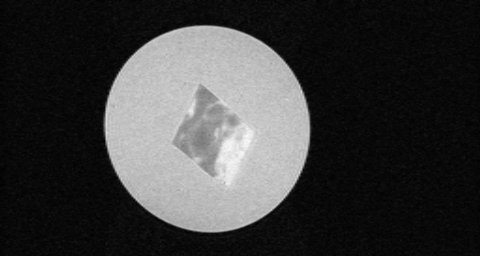
\includegraphics[scale=0.3]{13_1.jpg}
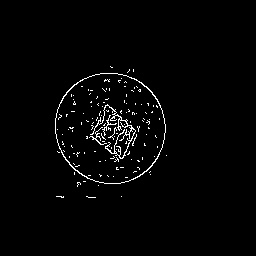
\includegraphics[scale=0.3]{edge(60,80)13_1.jpg}

Original Image \hspace{25mm} $T_l$ = 60, $T_h$ = 80
\end{center}
\begin{center}
\includegraphics[scale=0.3]{edge(60,115)13_1.jpg}
\includegraphics[scale=0.3]{edge(90,115)13_1}

$T_l$ = 60, $T_h$ = 115 \hspace{20mm} $T_l$ = 90, $T_h$ = 115
\end{center}

Due to the fact that it is left to the analyst to determine the limiting gradient values, it is worth noting the effects of altering the threshold values $T_h$ and $T_l$.
As one increases the upper-threshold $T_h$, fewer pixels will satisfy the criteria for being a strong edge, so there will be fewer edges produced in the final image $\cite{16}$.
However, as the lower-threshold $T_l$ is increased, fewer pixels will satisfy the condition for being a weak edge, so the edges that are rendered will possess lengths that are much smaller $\cite{17}$.
The degree to which the threshold values are changed depends on the context and desired output of our edge detection, and thus will need to be fine-tuned. 

We can briefly verify the consequences of altering the thresholds by observing the four images of manganese-based contrast agent above. The original image is then processed through Canny edge detection with gradient threshold values of 60 for lower bound, 80 for upper bound. By raising the upper bound to 115, the strong pixels that fall below a gradient value of less than 115 are removed, so there are now fewer edges being rendered. By raising the lower bound to 90, the length of the resulting edges is smaller because there is a higher metric to filter the weak pixels adjacent to strong ones. Both increases to the thresholds yield a fewer amount of edges, but the reasons for the decrease in pixelated edges are different.

\subsection{Image Registration}

One of the nuances of biomedical imaging analysis is having to establish a uniform coordinate system for any two images we wish to compare. In an ideal scenario, all images taken of a patient would be oriented in such a way that, if one were to stack the images on top of each other, the body and organs would be perfectly aligned. However, this is obviously not the case: as the scanner produces multiple images the patient may slightly move or turn, creating an image with features that are uncentered or rotated. This complicates comparing rendered images, so it is imperative that both images are properly transformed so that their relevent features are aligned in the same coordinate system. 

\newpage
\subsection{Technologies and Frameworks}

This section will briefly cover the most relevant technologies used in constructing and designing the image-processing environment I have created.

\singlespacing

\subsubsection{VirtualBox}


\begin{wrapfigure}{L}{0.5\textwidth}
\centering
\includegraphics[width=0.15\textwidth]{Virtualbox_logo.png}
\caption{VirtualBox}
\end{wrapfigure}

VirtualBox is an open-source memory-hosted (as opposed to hardware-hosted) hypervisor developed by Innotek GmbH in 2007 and acquired by Oracle Corporation in 2010 $\cite{18}$. 
It is cross-platform compatible as long as the machine adheres to an x86 CPU architecture $\cite{18}$. VirtualBox allows the user to support and manage their own virtual machines running on their host computer. Virtualization is a useful technique because it offers an easy and streamlined solution to shipping software packages and systems. Virtualization also offers the user the ability to spin up multiple operating systems and a more stable and isolated environment for testing and stressing of software and systems. To this day, Vagrant continues to grow and garner community support through the Open Source Project $\cite{18}$.

\begin{wrapfigure}{R}{0.2\textwidth}
\begin{center}
\includegraphics[width=0.15\textwidth]{Vagrant.png}
\end{center}
\end{wrapfigure}

\subsubsection{Vagrant}

Vagrant is another open-source software written in Ruby and used for configuring virtual environments $\cite{19}$.. It was developed and released by HashiCorp in 2010 and continues to grow. Vagrant is commonly used as a wrapper in conjunction with virtualization software such as VirtualBox or VMWare. It aims to solve the issue of software refusing to cooperate with a user's unique system or machine for whatever reason. Basically, if it works on one person's machine, it should work on anybody else's so long as they have Vagrant installed. Some of the benefits of using Vagrant include a streamlined, automated provisioning as well as effortless portability $\cite{19}$. 

\subsubsection{Conda}

Conda is an open-source package and environment management system developed by Continuum Analytics and released in 2014 $\cite{20}$. Although it is written primarily in and for Python, it can support packages designed for multiple languages, such as R or C++. It allows the user to seamlessly install package binaries from well-maintained repositories as well as interchangeably switch between versions of software for dependency-integrity. 

\subsubsection{OpenCV}

\begin{wrapfigure}{L}{0.2\textwidth}
\begin{center}
\centering
\includegraphics[width=0.15\textwidth]{OpenCV.png}
%\caption{OpenCV}
\end{center}
\end{wrapfigure}


OpenCV (Open Source Computer Vision) is a cross-platform ensemble of computer-vision functions originally developed by Intel in 1999 in Nizhny Novgorod, Russia $\cite{21}$. It is entirely written in C/C++ and has interfaces for C, C++, Python, Java and MATLAB $\cite{21}$. The project was created as an initiative to further progress computationally intensive processes (such as ray-tracing) by offering a portable, free library of optimized functions that adhered to a well-defined infrastructure which developers could collaborate on. The library offers many vision-applications and statistical learning models such as feature extraction, motion-tracking, classification and learning-trees $\cite{21}$. There was a second release of OpenCV in 2008. Since 2012, the project has been maintained by a non-profit foundation OpenCV.org. 

OpenCV is widely used throughout the globe for a variety of applications. Thanks to its efficient real-time processing power, OpenCV is used for purposes such as detecting swimming pool drownings, intrusions in surveillance video, product quality assurance and rapid, instantaneous facial recognition. It has approximately 2500 optimized computer-vision and machine learning algorithms, with over 9 million downloads worldwide $\cite{21}$.

\subsubsection{ImageJ}

ImageJ is an open-source java-based image-processing software developed by the National Institute of Health $\cite{22}$. It was released in 1997 as a successor to the freeware image analysis software titled NIH Image. It contains an extensible toolset for image manipulation and can accommodate most image formats (.GIF, .JPEG, .PNG, .BMP). By utilizing an in-memory stack of images per window, it can quickly perform such calculations as contrast manipulation, convolution, Fourier analysis, and smoothing/sharpening $\cite{22}$. ImageJ was used for sample-quality inspection after their preparation. Currently, it is one of the fastest java-written image-processing softwares to exist, clocking in at 40 million pixels per second, or an entire 2048x2048 image in 0.1 seconds $\cite{22}$.

\end{section}


\newpage
\begin{section}{Methods}

This section will provide a detailed explanation of the innerworkings of the system I have created to perform edge-detection on the manganese chloride images. There will also be a step-by-step documentation of the preparation and synthesis of the imaged samples.


\subsection{Design of Image-Analysis System}

This section will walk through the construction and design of the image-analysis system I have created. I will elaborate on the function and purpose of the system.

\subsubsection{Benefits and Utility}

As the reader may have noticed in the subsection detailing the relevant technologies, every single software listed was categorized as open source software. One of the most stifling drawbacks of depending on other image-analysis software (such as MATLAB) is that the software is typically labeled as proprietary, or closed-source software. This poses several issues: 1) researchers and scientists may not have the resources to purchase a legal license to use the software 2) the code which the algorithms are implemented with is not available to the public, and 3) collaborative development is non-existent outside the owner of the license. By including only open source technologies, I have created a completely free and easily-accessible tool for other researchers to perform automated edge-detection on a corpus of images. Thanks to the layer of abstraction and hardware-isolation provided by virtualization software such as Vagrant and VirtualBox, the system is not heaviliy reliant on the user-machine's dependencies. Thus the system is effortless to deploy for whomever would be interested. 

\subsubsection{An Overhead View}

Below is a simple diagram that briefly describes the interactions and encapsulation of all the software my system requires.

\begin{center}
\includegraphics[scale=0.35]{SystemDesign.png}
\end{center}

With VirtualBox running, the Vagrant environment can be initialized if it had not been previously instantiated. The virtual machine can be called or killed whenever the user requires its services. If the virtual environment has not been provisioned, the first thing Vagrant will do is pull an Ubuntu 14.04 operating system for our environment to run on. Several bash shell scripts will then be called to configure the system. This includes building target/result directories for our image, as well as installing libraries and packages like Conda and OpenCV. 

After all dependencies have been installed and verified to be working, the user may SSH (secure shell) into the Vagrant environment for script-execution, any minor tweakings, or exploration. Ingesting the images of interest is very simple and requires only a placing a folder of images into a synced directory on the host machine. Once the images of interest have been injected, the user simply executes a python script to analyze all images within the target directory and store the results in a result directory. The resulting images are automatically saved to the synced folder on the host machine.

Anybody can download this system by simply cloning the project's repository from Github and following the provided README.md file that walks the user through set-up and use.

\subsection{Synthesis of Manganese Chloride Contrast Agents}

To determine which concentrations of manganese chloride to use for our testing, we first began by taking both $T_1$ and $T_2$ weighted MRI scans of varying concentrations of contrast agent and distilled water in 10mL vials. Concentrations could vary anywhere from 0.01 to 5 parts manganese chloride to water. It was then left to the discretion of the lab-worker to select a range of concentrations that best yielded a brighter image for $T_1$ imaging and a darker image for $T_2$. On the 5th of April, 2016, Xiaowan Zheng and I selected 6 concentrations of 2, 1, 0.5, 0.2, 0.1, and 0.08 as candidate concentrations for a second round of imaging. All 6 concentrations proved to be hopeful contrast agents in that they produced brighter and darker images for $T_1$ and $T_2$.\\

After selecting our 6 concentrations, duplicates contrast agents were produced in amounts of 20mL. With a 100 $u$Molar solution of manganese chloride we then recreated the concentrations found to be promising by once again mixing with parts of distilled water. The concentration-breakdowns of each contrast agent are below:

\begin{center}
    \begin{tabular}{ | l | l | p{2cm} |}
    \hline
    Concentration & mL of $MnCl_2$ & mL of $H_2O$ \\ \hline
    2.0 & 0.4 mL & 19.6 mL  \\ \hline
    1.0 & 0.2 mL & 19.8 mL \\ \hline
   0.5 & 0.1 mL & 19.9 mL \\ \hline
   0.2 & 0.05 mL & 19.95 mL \\ \hline
   0.1 & 0.02 mL & 19.98 mL \\ \hline
   0.08 & 0.8 mL of 2uM & 19.2 mL \\ \hline
    \end{tabular}
\end{center}

Once all concentrations had been portioned out, each contrast agent was mixed with heated liquid agar. Because agar solidifies at room temperature, stacks of contrast agents with varying concentrations can be layered on top of one another. First 200 mL of distilled $H_2 O$ were mixed with 6 grams of agar to create a solution of 3 percent pure agar. The agar solution was then heated in a microwave until the solution was homogeneous enough that the agar particles were distributed uniformly enough. To remove air bubbles from the agar, the solution was placed in a heat bath. Air bubbles and other impurities could potentially ruin our samples' images, so it was imperative to remove them to the best of our ability.\\

\begin{center}
\includegraphics[scale=0.5]{6tray.png}
\end{center}

Once our solution of agar was as homogeneously uniform as possible, 5 mL of each contrast agent were combined with 5 mL of liquid agar. Each mixture was placed into one of 6 wells and left to solidify. The photograph above shows mixtures, from right to left, of concentrations 2, 1, 0.5, 0.2, 0.1, 0.08 (empty). Once the mixtures hardened, "cubettes" (small cubes) of contrast agent were sliced from the well to be embedded into our final sample in order to observe their effectiveness as $T_1$ and $T_2$ contrast agents.

Our 50 mL vial was then filled with hardened agar mixed with contrast agents of different concentrations. The first layer at the bottom of the vial was filled with pure agar. This first layer provided the ground that the first cubette of manganese chloride rested upon. To extract the cubette, a precision knife was used to partition the gel-like agent into many sections. By inspection, the cubette that was the most uniform in size and substance, meaning no bubbles, tears, or miscellaneous impurities, was selected as the candidate cubette. The first candidate cubette of concentration 2 was placed on the level of pure agar. The space surrounding the candidate cubette was filled with pure agar and left to solidify, providing the next level for the sequential cubette to sit on. It is important to note that the surrounding agar had to provide a buffer between each cubette, so each cubette was completely submerged in surrounding agar. This process was repeated until we had selected candidate cubettes from each concentration. The remainder of the vial was filled with agar and ready for MRI. \\

%Include side by side of layer by layer image
\begin{center}
\includegraphics[scale=0.4]{sample.png}
\hspace{25mm}
\includegraphics[scale=0.5]{5layers.jpg} \\
\small{A schematic of the 50 mL vial [8], and a cross-sectional image of a sample}
\end{center}

\end{section}

\newpage
\begin{section}{Results}
%Conc 1: 	T1_21 TE = 8.6984, TR = 940
%Conc 1: 	T2_19 TE = 12, TR = 4200
%Conc 0.1: 	T1_16 TE = 8.6984, TR = 940
%Conc 0.1: 	T2_14 TE = 12, TR = 4200
\subsection{Image Sets}

%Talk about sets of samples, parameters, images (mine and ImageJ's), and why there are lack of results
The samples used to perform edge-detection were synthesized using the aforementioned method on November 11th, 2015. There were only 4 concentrations of manganese chloride included in the set of weighted images (1, 0.1, 0.04, 0.004). Also included is a control pair of weighted images that displays only a slice of pure agar viewed from above. All $T_1$ weighted images were taken with $T_E$ = 8.6984ms, $T_R$ = 940ms. All $T_2$ weighted images were taken with parameters $T_E$ = 12.00ms, $T_R$ = 4200ms. It is important to clarify that this batch of images does not accurately represent the intended effect of the contrast agent. Instead of all concentrations showing a brighter signal with $T_1$ and a darker signal with $T_2$, some sets show no observable contrast difference. It may also be the case that $T_2$ weighted images actually show an increased brightness, while some $T_1$ weighted images show a darker signal. Therefore, this dataset was only used to deduce the validity of samples via Canny edge-detection, and not for determining concentration efficiency. 

Because our only set of manganese chloride concentrations has been considered unfit for determining their effectiveness as $T_1$ and $T_2$ contrast agents, representative images were created using the image-editing software GIMP. Several sets of images were created to emulate the agents' intended effects. All images were created using a template to ensure uniform dimensions. Any discrepancies between $T_1$ and $T_2$ images would negatively influence the quantitative assessment of a concentration's suitability as an agent. When creating the collection of artificial images, specific gray-scale quantities were taken to ensure that some concentrations were deemed more suitable than others. The surrounding agar was always created using a grayscale value of 195 and an airbrush with pixel shade of 210 as a way to simulate noise. The airbrush was separately applied to each image to emulate the agar's unexpected response to $T_1$ and $T_2$ weighting in order to demonstrate the necessity for normalizing our cubettes' measured efficiency. 

For $T_1$ weighting, all cubette regions were filled with shades that were considerably brighter than the surrounding agar. $T_2$ images were filled with shades that were noticeably darker than the surrounding agar. Sets of images were constructed such that each pair varied slightly in contrast-difference. This was done by shading one or both cubette regions with slightly greater or smaller pixel-values. An airbrush was also applied to cubette regions to emulate noise and agent non-uniformity.

The set of agents created on April 5th, 2016 (concentrations 2, 1, 0.5, 0.2, 0.1, and 0.08) were imaged shortly after their synthesis. Because the produced images did not display any significant changes in brightness, they were ultimately discarded as a failed batch. This set of images will neither be included nor discussed. 

\subsection{Determining sample "goodness" with edge-detection}

A valid sample will obey the two following clauses: 

\singlespacing
\begin{enumerate}
\item The sample's cubettes are uniform in consistency and contain no obstructive impurities
\item The sample's cubettes expected to show an enhanced signal do exhibit a change in pixel-brightness
\end{enumerate}
\doublespacing

A sample that fails to meet the above requirements can not be considered useful. If the cubette appears non-uniform and afflicted with multiple impurities, then it cannot be determined whether or not the contrast agent is responsible for the enhanced signal. An impurity can be a tear in the gel-cubette, a trapped air-bubble that was caught between the surrounding agar and cubette during insertion, or an unexpected suspended particle that was not intended to be included. The synthesis procedure aims to minimize the possibility for impurities: the agar is distributed as uniformly as possible to ensure no clumps of particles and the air-bubbles are removed with the use of a heat bath. All impurities that would significantly influence the goodness of a sample are easily detected by Canny edge detection. However, the true difficulty lies in distinguishing anomalies from background noise. A careful application of edge-detection will determine whether or not a pair of images satisfies both conditions. 

\subsubsection{Determining Optimal Thresholds} %Use Regression To Self-Balance Thresholds (talk in conclusion)

The first obstacle to hurdle when applying Canny edge-detection to a sample's set of images is to find a pair of lower-bound and upper-bound thresholds that sufficiently extract the interesting features and remove unnecessary image-noise. If thresholds are set too low, edge-detection will incorrectly label many pixel-gradients as possible strong or weak edges. On the other end of the spectrum, thresholds set too high will remove all interesting edges of our image. This was done by inspecting multiple edge-images with varying thresholds until a desirable image was created. Edge-detection was first applied to images of pure agar to find the right parameters to filter out false edges generated in regions absent of features.

\newpage
\begin{center} \underline{Edge-Detection of Pure Agar ($T_2$ weighted)} \end{center}
\begin{flushleft}
\includegraphics[scale=0.3]{pure_agar_T2.jpg}				\hspace{2cm}$T_2$-weighted image with no detection
\includegraphics[scale=0.3]{noisy_pure_agar_(60,80).jpg}	\hspace{2cm}With $T_L$ = 60, $T_H$ = 80
\includegraphics[scale=0.3]{pure_agar_(90,115).jpg}			\hspace{2cm}With $T_L$ = 90, $T_H$ = 115
\end{flushleft}

The above images illustrate the influence the thresholds have over the edge-detection output. By inspection, one can see there is nothing of interest inside the sample. By setting our hysteresis thresholds too low ($T_L$ = 60, $T_H$ = 80), a lot of false edges are generated as seen in the second image. Only until we raise the thresholds to $T_L$ = 90 and $T_H$ = 115 do we remove lots of unwanted noise. It was then decided that thresholds $T_L$, $T_H$ from between 70 and 120 would produce desirable outputs. All of the edge-images in the following sections will have been produced from thresholds falling between this appropriate range.

\subsubsection{Satisfying Cubette Uniformity}

Now that an acceptable range of thresholds has been created, edge-detection is applied to determine the uniformity of cubettes. By observing the rendered features and edges of the algorithm's output, the researcher can determine the severity of the imperfections or anomalies. Two $T_2$-weighted images, one with an agent concentration of 0.004 and the other with 0.04, have been selected to demonstrate this exercise. It is important to note that the $T_2$ image for concentration 0.04 actually shows a brighter signal, instead of an expected darker image. Regardless the characteristics of the cubette-region are well-suited for this demonstration. The images may be found below:

\begin{center}
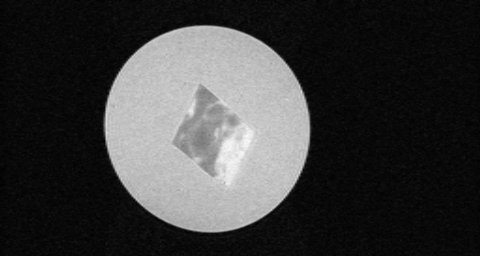
\includegraphics[scale=0.4]{13_1.jpg}
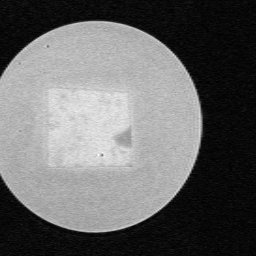
\includegraphics[scale=0.4]{19_1.jpg}\\
\small{Left: $T_2$ image of conc. 0.004, Right: $T_2$ image of conc. 0.04}
\end{center}

It is evident that both images contain cubettes that aren't completely homogeneous. In hopes of detecting the impurities in the cubettes, a round of edge-detection is performed. Below is a subset of the produced images:

\begin{center}
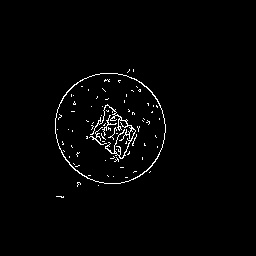
\includegraphics[scale=0.4]{edge(60,90)13_1.jpg}
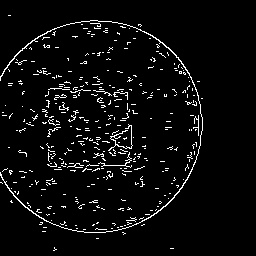
\includegraphics[scale=0.4]{edge(60,90)19_1.jpg}\\
\includegraphics[scale=0.4]{edge(60,115)13_1.jpg}
\includegraphics[scale=0.4]{edge(60,115)19_1.jpg}\\
\small{Top Row: $T_L$ = 60, $T_H$ = 90} \hspace{1mm} \small{Bottom Row: $T_L$ = 60, $T_H$ = 115}
\end{center}

For concentration 0.004, the anomalies may be defined as the rapidly varying ares of light and dark pixels. With respect to the image for sample-concentration 0.04, the single dark speck on the border of the cubette may be labeled as an impurity. In all four edge-images, the cubette and its anomalies were detected and labeled as regions of significant intensity-change. By increasing the upper threshold from 90 to 115, the number of strong edge-pixels was reduced and the amount of noise surrounding the cubette diminished. Despite this increase of the upper threshold, the impurities were still detected and rendered. Thus it is safe to say that the bottom row's edges contained within the cubette's boundaries represent abnormalcies that are prominent enough to warrant the samples as non-homogeneous. The degree of non-uniformity to which we may characterize the sample with concentration 0.004 is much larger than that of the sample with concentration 0.04. This may be verified by comparing the number of pixels and edges between concentrations 0.004 and 0.04.

So it has been illustrated how edge-detection can be applied to detect cubette-anomalies. In order to demonstrate how homogeneous and uniform a cubette can appear, another iteration of edge-detection has been performed to a $T_1$-weighted image. The original and processed images may be found below:

\begin{center}
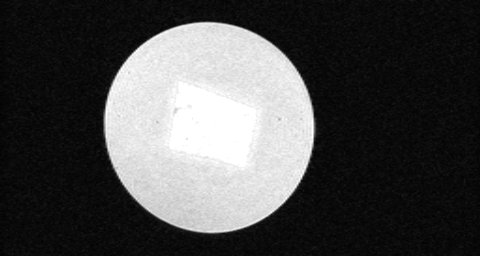
\includegraphics[scale=0.4]{20_2.jpg}
\includegraphics[scale=0.4]{edge(60,85)20_2.jpg}\\
\small{Left: $T_1$ image of conc. 0.1} \hspace{13mm} \small{Right: $T_L$ = 60, $T_H$ = 85}
\end{center}

What is most surprising about the above images is that the cubette was so homogeneous and void of impurities that the surrounding region of pure agar produced more edges than the contrast agent itself. In order to affirm a cubette's uniformity, the region confined within the cubette's boundaries must be nearly void of any detected edges. It is not required for the cubette to "outperform" its surrounding region of agar, but doing so certainly speaks volumes of how pure and anomaly-free the cubette can be.

\subsubsection{Detecting Well-Defined Cubette Boundaries}

Due to the likelihood that a $T_1$ or $T_2$-weighted image may fail to produce a brighter or darker signal, it is imperative to verify that the sample's concentrations that ought to produce an image contrast do so. This can be done by inspecting the edge-detection's produced boundaries. The contiguity of the cubette's perimeters and their resilience to an increase in hysteresis-thresholds will determine how well the cubette is defined. To demonstrate how the boundaries of one concentration's cubette may differ from other concentrations' cubette's, four edge-images that were previously introduced are collected on the following page:

\newpage
\begin{center} \underline{Locating the Cubette with Edge-Detection} \end{center}
\begin{flushleft}
\includegraphics[scale=0.26]{pure_agar_(90,115).jpg}		\hspace{0.5cm}\small{Pure Agar $T_2$ ($T_L$:90,$T_H$:115): No Boundaries}
\includegraphics[scale=0.26]{edge(60,115)19_1.jpg}			\hspace{0.5cm}\small{Conc. 0.04 $T_2$ ($T_L$:60,$T_H$:115): Sparse Boundaries}
\includegraphics[scale=0.26]{edge(60,115)13_1.jpg}			\hspace{0.5cm}\small{Conc. 0.004 $T_2$ ($T_L$:60,$T_H$:115): Well-Defined Boundaries}
\includegraphics[scale=0.26]{edge(60,85)20_2.jpg}			\hspace{0.5cm}\small{Conc. 0.1 $T_1$ ($T_L$:60,$T_H$:85): Well-Defined Boundaries}
\end{flushleft}

The first image consists of only the circumference of the sample's container. Therefore there should be no other detected edges in the produced image and is expected for samples containing no cubettes. The edge-image derived from the $T_2$-weighted sample of concentration 0.04 shows a rendered object that is sparsely connected: sides of the cubette do not converge at their supposed vertices. The $T_2$-weighted image of concentration 0.004 shows a considerably more well-connected perimeter. The $T_1$-weighted image of concentration 0.1 also shows a well-defined perimeter, but not to the extent of the third image. Despite the fact that the third image's cubette includes many impurities while the fourth's does not, both images satisfy the condition that their cubette's produce a contrast in image-brightness. Meeting this requirement solely depends upon the perimeter generated by edge-detection.

Determining the resilience of the cubette's boundaries may be calculated by taking a quantitative metric (pixel-count, or edge-length) for many iterations of edge-detection with incrementing thresholds. The stronger the contrast in brightness produced by the contrast agent, the longer the cubette's edges will survive as the thresholds are raised. Plotting a count of white-pixels in the edge-image versus the values of the algorithm's thresholds could reveal something about the resilience of the cubette's edges. 

\subsection{Determining the most optimal $Mn-Cl_2$ Concentration}

We are interested in determining the most optimal concentration of contrast agent. "Optimal" would mean the concentration that excellently produces brighter images with $T_1$-weighting and darker images with $T_2$-weighting. It has been demonstrated that some concentrations yield resulting images that are either all brighter, all darker, or display no real influence on the image's intensity. This could either have been due the to contrast agent's concentration alone, or a poor choice in MRI parameters ({\em Echo-Time, Relaxation-Time, radio pulse frequency, etc.}). A concentration's efficiency for a specific set of parameters could be quantified as the difference in pixel-intensities from $T_1$ and $T_2$. Greater differences in intensities would signify an increased effectiveness for a concentration. The following sections will describe my solution to this problem, as well as obstacles I encountered.

\subsubsection{Assumptions \& Method}

In order to approach this problem, some assumptions must be made about our images. Their resolutions will appear following the description of the solution. The assumptions are as follows:

\singlespacing
\begin{enumerate}
\item The sample's cubettes of contrast agent are uniform in dimension
\item The sample's cubettes' locations do not deviate from each other
\item The sample's surrounding agar does not exhibit intensity-contrast
\end{enumerate}
\doublespacing

The first assumption is critical because it directly influences the metric on which we gauge the concentration's effectiveness. If one concentration's cubette covers more of the image than another concentration's cubette, then we could incorrectly label one concentration as more or less effective than its competitors. The second assumption makes the approach possible, because feature-extraction of this nature would be impossible if images were to be misaligned in their coordinate-planes. The third assumption removes the task of normalizing the result to verify the true efficiency of our concentrations. All assumptions are discussed in further detail later.

The Python file titled {\em findBestConcentration.py} in the {\em scripts} directory contains all the necessary calculations and functions to successfully determine the "most optimal" concentration given a set of $T_1$ and $T_2$ images. First, all images in the target-folder's subdirectories are loaded and paired according to their concentrations. For every pair of $T_1$ and $T_2$ images, the following is done:

\singlespacing
\begin{enumerate}
\item Extract N-horizontal pixel vectors from the center of both images (N is user-defined)
\item Apply a 1-D Gaussian convolution mask to further reduce noise for every pixel vector
\item For every horizontal pixel vector find the absolute value of the difference between its corresponding "sibling" pixel and store as a vector
\item Normalize this pixel-difference vector by removing the pixels produced by the agar's intensity contrast
\item Treat the vector of pixel-differences as a curve and calculate the area underneath the curve
\end{enumerate}

\doublespacing

The concentrations are then sorted according to their results from determining the area under their pixel-difference vector. The concentrations with the largest areas are recommended as an optimal contrast agent.

\subsubsection{Issues and Solutions}

As previously mentioned, the assumptions made to ensure this solution's confidence and precision were 1) the cubettes do not vary in size from one concentration to another, 2) the cubettes do not appear to move from image to image, and 3) the pure agar does not experience notable intensity-change. Their influence on the above approach for determining the best concentration levels will now be discussed, along with possible solutions.

The first assumption was formulated to remove the bias some concentrations would create when calculating the area under the curve. For larger cubettes of contrast agent, more area would lie underneath the pixel-difference curve and would thus yield a deceptively larger or smaller area. This augmented area would misrepresent the concentration's effectiveness, so the assumption is made that all cubettes are uniform. One potential approach to overcome this obstacle would be to standardize the region under which we calculate our area/efficiency. An application of 1-Dimensional Canny edge detection would be used to determine the locations along the pixel-difference vectors where intensity-transition is highest. These locations would represent where the pure agar turns into brighter or darker regions containing contrast agents. The boundaries surrounding the smallest regions would then be applied to all concentrations to ensure the areas under the curves would be taken over a uniform range. This would then represent a more realistic efficiency-score for our concentrations.

The second assumption was created to remove the necessity for image-registration. If two cubettes of the same concentration were slightly misaligned, then the calculated efficiency would not be an accurate representation. If it is assumed that the camera and/or sample does not move between $T_1$ and $T_2$ images, then it is no longer necessary to align the images. To resolve this issue, all pairs of images would be registered with respect to each other features and origins.

The third assumption requires the algorithm to account for unexpected brightness-contrast caused by surrounding agar. If for one concentration the agar had produced varying intensities, this would leave our concentrations' true efficiencies unnormalized. Because the surrounding agar is not uniform in brightness, this begs the question: Which values do we reduce our pixel-difference vector by? One approach may be to discretize and bin pixels outside the region of highest pixel-contrast and then reduce their influence on the cubette's pixel-contrast. This would result in a much more accurate and representative metric for concentration efficiency. 

\subsubsection{Results}

Because of the lack of sample sets with desirable characteristics (brighter image in $T_1$, darker image in $T_2$), the aforementioned algorithm was preformed on several sets of artificial, but representative sample-images created in GIMP. Some of the images can be seen below:

\begin{center}
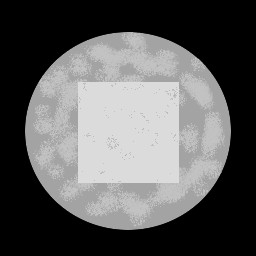
\includegraphics[scale=0.25]{T1.jpg}
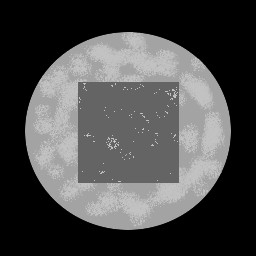
\includegraphics[scale=0.25]{T2.jpg}
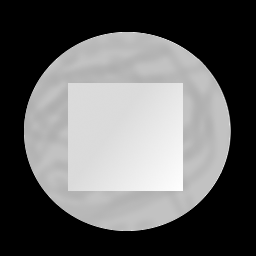
\includegraphics[scale=0.25]{T1*.png}
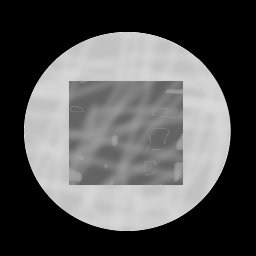
\includegraphics[scale=0.25]{T2*.png}
\end{center}
\begin{center}
\small{Two test sets of $T_1$ and $T_2$ images, (Set No. 2 $T_1$ and $T_2$, Set No. 3 $T_1$ and $T_2$)}
\end{center}

Line graphs representing the pixel-intensities for ideal $T_1$ and $T_2$ images were taken during testing and may be found below:

\begin{center}
\includegraphics[scale=0.35]{SingleSlice_Test3_T1.png}
\includegraphics[scale=0.35]{SingleSlice_Test3_T2.png}
\end{center}

Both slices of pixel-values were taken laterally along the middle of the image and interesect the regions of enhanced and reduced brightness. Both graphs belong to test set 3, as seen above. It is important to note that the surrounding agar does noticeably vary from $T_1$ to $T_2$, and was done so to demonstrate the necessity for normalizing the agents' contrast difference.

For smoothing the horizontal slices of pixels, a 1-D Gaussian Filter was selected with size 5 and $\sigma = 1.4$:

\begin{center}
$G_F = \frac{1}{159}
\begin{matrix}
[ 5 & 12 & 15 & 12 & 5 ]
\end{matrix}$
\end{center}
	
Once applied, the final pixel-difference vector represented by a line graph appeared like so:

\begin{center}
\includegraphics[scale=0.6]{Unnormalized_GF_Test3.png}
\end{center}

It is easy to see that because we left the vector unnormalized, regions of surrounding pure agar still influence the area underneath the curve. This demonstrates the necessity for determining the contribution to the efficiency-score made by the slight contrast in the agar. A 1-Dimensional application of Canny edge detection would yield a position-approximation for region boundaries. Because the intensity-gradient changes so dramatically around the region of transition, there would be no difficulty in isolating the region of agar from the cubette.

\end{section}

\newpage
\begin{section}{Conclusion}
\subsection{Discussion of Results}

Despite not having a large corpus of sample images for testing purposes, the aforementioned methods and solutions performed as expected. Rounds of Canny edge detection applied to actual sets of $T_1$ and $T_2$ images yielded valuable information. Edge detection demonstrated how the contiguity of cubette boundaries may vary as hysteresis thresholds are changed. Finding the sweetspot for threshold values proved itself possible: image-noise was sufficiently reduced and relevant features such as impurities and cubettes were still detected. Rendered images could verify the goodness of samples of contrast agents by detecting the anomalies within the cubette's boundaries. The strength of the contrast agents' enhanced signals could also possibly be determined by monitoring the resilience of the cubette's perimeters as threshold values are raised. These results demonstrated that a careful application of Canny edge detection could certainly further our exploration of manganese-based contrast agents in MRI. However one of the obstacles concerning this application of image-analysis is the difficulty of selecting a pair of threshold values that all samples agree upon. Some thresholds were better suited for one set of images, but did not produce ideal results for others. A potential solution for this shortcoming is a clever application of machine learning to train a model to distinguish image-noise from interesting features. This could potentially lead towards training models to determine the goodness of agent samples.

Because our images did not accurately represent the intended effects of manganese-chloride contrast agents, the methods for determining the most efficient concentration were applied to a smaller set of self-made images. However the methods were verified to work for future sets of sample images. In anticipation of our solutions' assumptions being broken, images would have to be properly registered to preserve the information stored in each sample's features. It would also be very feasible to create a work-around for non-uniform cubettes in case there is no reasonable method for synthesis identical samples. This could be done by using a 1-Dimensional application of Canny edge detection to determine the smallest cubette's dimensions and then applying these dimensions to all other samples. This would ensure a constant region of interest, thus yielding an accurate area-under-curve result. Our results also demonstrated the need to normalize our agent's contrast difference, but this should also be a very feasible issue to resolve.

Some of the issues that were responsible for 'bottlenecking' results were the slow rate at which sample sets were created and imaged. Due to its busy schedule, the MRI machine at the hospital was not always available to render images of our synthesized samples. The image-analysis system I created can accommodate many images, but it was never fed anything more than 15 concentrations. Images could also show disappointing results and were discarded. Reasons for unusual results could have been an incompatible selection of MRI parameters or an improperly synthesized sample set. Coupling this with the MRI machine's inavailability compounded the slow turnaround time of samples and images. It would have been ideal to have an easily accessible MRI machine for the research team to use whenever they wanted to. Nevertheless, the data used for this research was adequately representative of what future sample sets may look like.

\subsection{Future Applications}

Future endeavours concerning this research will take shape in two different ways: 1) the linux-based image-analysis environment will continue to be improved upon by myself in anticipation of more experimentation, 2) the research team at Georgetown University will continue investigating the properties of manganese-based contrast agents. I will continue adding, refactoring, and designing new ways to digitally gain information from image sets. I invite anyone with Python knowledge and an interest in image-processing to experiment or deploy the system. The entire project is currently public and hosted on Github.com at \\
{\em https://github.com/patrickstocklin/SeniorThesis} and can be effortlessly downloaded and instantiated.

The image-processing environment can be improved upon in several ways. One direction the project could head in is towards the applications of machine learning. Machine learning could assist the research effort by learning to classify good and bad pairs of images. By building a classifier model through training, the efficiency of the classification would be augmented with the knowledge of previous samples' characteristics. Another area the project could improve upon is incorporating other feature-extraction techniques to learn more information about our contrast agent's effectiveness. Other potentially useful techniques include Hough Line and Hough Circle Transforms, which are aimed at recognizing patterns like lines and arcs found in images. Implementations of both algorithms can be found in OpenCV, so incorporating them into the application would be of no issue. Machine learning could also train the system to better identify the strength contrast difference for given concentrations by learning how to weight the difference in pixel-count as a function of changing edge-detection thresholds. This would help separate the noise in the agar from the interesting information contained in the boundaries of the contrast agents. The system could also be forced to perform image registration of all incoming sets of images using feature extraction. Doing so would significantly minimize the error of the model in the scenario of unintended feature-misalignment. All of the aforementioned applications from the system could benefit from are feasible and promising.

\end{section}

\newpage
\singlespacing
\begin{thebibliography}{9}

%Good
\bibitem{1}
Formica D, Silvestri S (April 2004). {\em Biological effects of exposure to magnetic resonance imaging: an overview}. Biomed Eng Online 3: 11. 

%Good
\bibitem{2}
American Society of Neuroradiology, 2013. {\em ACR-ASNR Practice Guideline for the Performance and Interpretation of Magnetic Resonance Imaging (MRI) of the Brian}.

%Good
\bibitem{3}
McRobbie D., et al. MRI, {\em From picture to proton}. 2003

%Good
\bibitem{4}
Malcolm H. Levitt (2001). {\em Spin Dynamics: Basics of Nuclear Magnetic Resonance}. Wiley.

%Good
\bibitem{5}
Koretsky, Alan P.; Silva, Afonso C. (2004). {\em Manganese-enhanced magnetic resonance imaging (MEMRI)}. NMR in Biomedicine 17 (8): 527–31

%Good
\bibitem{6}
Lin, Yi-Jen; Koretsky, Alan P. (1997). {\em Manganese ion enhances T1-weighted MRI during brain activation: An approach to direct imaging of brain function}. Magnetic Resonance in Medicine 38 (3): 378–88.

%Good
\bibitem{7}
Michele Pablico-Langisgan, William Hickling, Emily Japp, Olga Rodriguez, Anup Ghosh, Chris Albanese, Maki Nishida, Edward Van Keuren, Stanley Fricke, Norman Dollahon, Sarah Stoll. 2013, Magnetic Nanobeads as Potential Contrast Agents for Magnetic Resonance Imaging, {\em American Chemical Society}, v.7 no.10, p.9040-9048.

%Good
\bibitem{8}
Joseph N. York, Christopher Albanese, Olga Rodriguez, Yi-Chien Lee, Marian Ackun-Farmmer, Edward Van Keuren. 2014, The Effects of Particle Shape and Size on T2 Relaxation in Magnetic Resonance Imaging. {\em Journal of Biomedical Nanotechnology}, Vol. 10, p.3392-3396.

%Good
\bibitem{9}
Introduction to Computer Vision and Image Processing - Luong Chi Mai, Department of Pattern Recognition and Knowledge Engineering

%Good
\bibitem{10}
Image Editing in the contour domain - James Elder and Richard Goldberg, IEEE Transactions on PAMI

%Good
\bibitem{11}
A Survey and Evaluation of Edge Detection Operators Application to Medical Images - Hanene Trichili, Mohamed-Salim Bouhlel, Nabl Derbel, Lotfi Kamoun, IEEE, 2002

%Good
\bibitem{12}
D. Marr and E. Hildreth. {\em Theory of edge detection}. Proc. Royal Soc. London, 207:187–217, 1980

%Good
\bibitem{13} 
John Canny, {\em A Computational Approach to Edge Detection}. IEEE Computer Society, 1986

%Good
\bibitem{14}
D. Marr and E. Hildreth. {\em Theory of edge detection}. Proc. Royal Soc. London, 207:187–217, 1980

%Good
\bibitem{15}
Trucco, Verri. {\em Introductory Techniques for 3-D Computer Vision}, Prentice Hall, 1998.

%Good
\bibitem{16}
R. Deriche, Using Canny's criteria to derive a recursively implemented optimal edge detector, Int. J. Computer Vision, Vol. 1, pp. 167–187, April 1987.

%Good
\bibitem{17}
Statistical Edge Detecton: Learning and Evaluating edge cues - Scott Konishi, Alan Yuille, James Coughlin, and Song Chun Zhu, IEEE Transactions on PAMI

%Good
\bibitem{18}
VirtualBox Manual, Copyright© 1995-2014 Oracle and/or its affiliates. All rights reserved: https://www.virtualbox.org/manual/ch01.html

%Good
\bibitem{19}
Vagrant Documentation, HashiCorp: https://www.vagrantup.com/about.html

%Good
\bibitem{20}
Conda Documentation, Continuum-Analytics: http://conda.pydata.org/ pydata.org. (Retrieved 9 April 2015)

%Good
\bibitem{21} 
OpenCV Documentation, OpenCV.org: http://opencv.org/about.html

%Good
\bibitem{22}
Schneider CA, Rasband WS, Eliceiri KW (2012). {\em NIH Image to ImageJ: 25 years of image analysis}. Nat Methods 9 (7): 671–675.

\bibitem{23}
S. Agaian, A. Almuntashri. 2009. {\em Noise-Resilient Edge Detection Algorithm for Brain MRI Images}. 31 Annual International Conference of the IEEE EMBS, MN, U.S.A., September 2-6, 2009.
% \bibitem{1}
% Michele Pablico-Langisgan, William Hickling, Emily Japp, Olga Rodriguez, Anup Ghosh, Chris Albanese, Maki Nishida, Edward Van Keuren, Stanley Fricke, Norman Dollahon, Sarah Stoll. 2013, Magnetic Nanobeads as Potential Contrast Agents for Magnetic Resonance Imaging, {\em American Chemical Society}, v.7 no.10, p.9040-9048.

% \bibitem{2}
% Trucco, Verri. {\em Introductory Techniques for 3-D Computer Vision}, Prentice Hall, 1998.

% \bibitem{3}
% Introduction to Computer Vision and Image Processing - Luong Chi Mai, Department of Pattern Recognition and Knowledge Engineering

% \bibitem{4}
% John Canny, {\em A Computational Approach to Edge Detection}. IEEE Computer Society, 1986

% \bibitem{5}
% A Survey and Evaluation of Edge Detection Operators Application to Medical Images - Hanene Trichili, Mohamed-Salim Bouhlel, Nabl Derbel, Lotfi Kamoun, IEEE, 2002

% \bibitem{6}
% Image Editing in the contour domain - James Elder and Richard Goldberg, IEEE Transactions on PAMI

% \bibitem{7}
% Statistical Edge Detecton: Learning and Evaluating edge cues - Scott Konishi, Alan Yuille, James Coughlin, and Song Chun Zhu, IEEE Transactions on PAMI

% \bibitem{8}
% Learning to Detect Natural Image Boundaries using Local Brightness, Color, and texture cues - David Martin, Charless Fowlkes, and Jitendra Malki, IEEE Transactions on PAMI

% \bibitem{9}
% William E. Green, Edge Detection Tutorial (2002), Drexel University: $http://dasl.mem.drexel.edu/alumni/bGreen/www.pages.drexel.edu/_weg22/edge.html$

% \bibitem{10}
% D. Marr and E. Hildreth. {\em Theory of edge detection}. Proc. Royal Soc. London, 207:187–217, 1980

% \bibitem{11}
% R. Deriche, Using Canny's criteria to derive a recursively implemented optimal edge detector, Int. J. Computer Vision, Vol. 1, pp. 167–187, April 1987.

% \bibitem{12}
% Liu Cai,  {\em A  kind  of  advanced  Sobel  image  edge detection  algorithm}, Guizhou Industrial College Transaction (Natural Science Edition), 2004, 77-79. 

% %%%York Paper
% \bibitem{13} 
% Joseph N. York, Christopher Albanese, Olga Rodriguez, Yi-Chien Lee, Marian Ackun-Farmmer, Edward Van Keuren. 2014, The Effects of Particle Shape and Size on T2 Relaxation in Magnetic Resonance Imaging. {\em Journal of Biomedical Nanotechnology}, Vol. 10, p.3392-3396.

% %%%Kobayashi and Otsu Image Gradients
% \bibitem{14}
% Takumi Kobayashi and Nobuyuki Otsu, {\em Image Feature Extraction Using Gradient Local Auto-Correlations}. National Institute of Advanced Industrial Science and Technology, 2008. Springer-Vergal, Berlin.

% %%%MRI Sources
% \bibitem{15}
% Formica D, Silvestri S (April 2004). {\em Biological effects of exposure to magnetic resonance imaging: an overview}. Biomed Eng Online 3: 11. 

% \bibitem{16}
% American Society of Neuroradiology, 2013. {\em ACR-ASNR Practice Guideline for the Performance and Interpretation of Magnetic Resonance Imaging (MRI) of the Brian}.

% %%%T_1/T_2 Sources
% \bibitem{17}
% McRobbie D., et al. MRI, {\em From picture to proton}. 2003

% \bibitem{18}
% Malcolm H. Levitt (2001). {\em Spin Dynamics: Basics of Nuclear Magnetic Resonance}. Wiley.

% %Manganese Chloride Sources
% \bibitem{19}
% Koretsky, Alan P.; Silva, Afonso C. (2004). {\em Manganese-enhanced magnetic resonance imaging (MEMRI)}. NMR in Biomedicine 17 (8): 527–31

% \bibitem{20}
% Lin, Yi-Jen; Koretsky, Alan P. (1997). {\em Manganese ion enhances T1-weighted MRI during brain activation: An approach to direct imaging of brain function}. Magnetic Resonance in Medicine 38 (3): 378–88.

% %%%ImageJ Sources
% \bibitem{21} 
% Eliceiri K, Rueden C (2005). {\em Tools for visualizing multidimensional images from living specimens}. Photochem Photobiol 81 (5): 1116–22. 

% \bibitem{22}
% Schneider CA, Rasband WS, Eliceiri KW (2012). {\em NIH Image to ImageJ: 25 years of image analysis}. Nat Methods 9 (7): 671–675.

% %%%VIRTUAL BOX SOURCES
% \bibitem{23}
% VirtualBox Manual, Copyright© 1995-2014 Oracle and/or its affiliates. All rights reserved: https://www.virtualbox.org/manual/ch01.html

% %%%Vagrant SOURCES
% \bibitem{24} Vagrant Documentation, HashiCorp: https://www.vagrantup.com/about.html

% %%%CONDA SOURCES
% \bibitem{25} Conda Documentation, Continuum-Analytics: http://conda.pydata.org/ pydata.org. (Retrieved 9 April 2015)

% %%%OPENCV SOURCES
% \bibitem{26} OpenCV Documentation, OpenCV.org: http://opencv.org/about.html

\end{thebibliography}


\end{document}


